\subsection{Time Series Decomposition}
\label{decomp}

Concerning the time table in Figure \ref{f:timetable}, a seasonal demand
    pattern is inherent to both horizontal and vertical time series.
First, the weekday influences if people eat out or order in with our partner
    receiving more orders on Thursday through Saturday than the other four
    days.
This pattern is part of both types of time series.
Second, on any given day, demand peaks occur around lunch and dinner times.
This only regards vertical series.
Statistical analyses show that horizontally sliced time series indeed exhibit
    a periodicity of $k=7$, and vertically sliced series only yield a seasonal
    component with a regular pattern if the periodicity is set to the product
    of the number of weekdays and the daily time steps indicating a distinct
    intra-day pattern per weekday.

Figure \ref{f:stl} shows three exemplary STL decompositions for a
    $1~\text{km}^2$ pixel and a vertical time series with 60-minute time steps
    (on the x-axis) covering four weeks:
With the noisy raw data $y_t$ on the left, the seasonal and trend components,
    $s_t$ and $t_t$, are depicted in light and dark gray for increasing $ns$
    parameters.
The plots include (seasonal) na\"{i}ve forecasts for the subsequent test day
    as dotted lines.
The remainder components $r_t$ are not shown for conciseness.
The periodicity is set to $k = 7 * 12 = 84$ as our industry partner has $12$
    opening hours per day.

\begin{center}
\captionof{figure}{STL decompositions for a medium-demand pixel with hourly
                   time steps and periodicity $k=84$}
\label{f:stl}
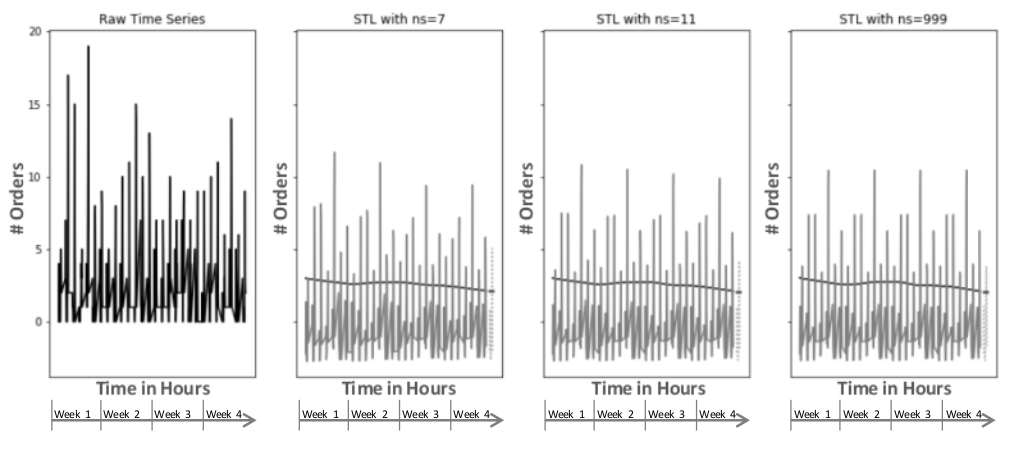
\includegraphics[width=.95\linewidth]{static/stl_gray.png}
\end{center}

As described in Sub-section \ref{stl}, with $k$ being implied by the
    application, at the very least, the length of the seasonal smoothing
    window, represented by the $ns$ parameter, must be calibrated by the
    forecaster:
It controls how many past observations go into each smoothened $s_t$.
Many practitioners, however, skip this step and set $ns$ to a big number, for
    example, $999$, then referred to as "periodic."
For the other parameters, it is common to use the default values as
    specified in \cite{cleveland1990}.
The goal is to find a decomposition with a regular pattern in $s_t$.
In Figure \ref{f:stl}, this is not true for $ns=7$ where, for
    example, the four largest bars corresponding to the same time of day a
    week apart cannot be connected by an approximately straight line.
On the contrary, a regular pattern in the most extreme way exists for
    $ns=999$, where the same four largest bars are of the same height.
This observation holds for each time step of the day.
For $ns=11$, $s_t$ exhibits a regular pattern whose bars adapt over time:
The pattern is regular as bars corresponding to the same time of day can be
    connected by approximately straight lines, and it is adaptive as these
    lines are not horizontal.
The trade-off between small and large values for $ns$ can thus be interpreted
    as allowing the average demand during peak times to change over time:
If demand is intermittent at non-peak times, it is reasonable to expect the
    bars to change over time as only the relative differences between peak and
    non-peak times impact the bars' heights with the seasonal component being
    centered around $0$.
To confirm the goodness of a decomposition statistically, one way is to verify
    that $r_t$ can be modeled as a typical error process like white noise
    $\epsilon_t$.

However, we suggest an alternative way of calibrating the STL method in an
    automated fashion based on our unified CV approach.
As hinted at in Figure \ref{f:stl}, we interpret an STL decomposition as a
    forecasting method on its own by just adding the (seasonal) na\"{i}ve
    forecasts for $s_t$ and $t_t$ and predicting $0$ for $r_t$.
Then, the $ns$ parameter is tuned just like a parameter for an ML model.
To the best of our knowledge, this has not yet been proposed before.
Conceptually, forecasting with the STL method can be viewed as a na\"{i}ve
    method with built-in smoothing, and it outperformed all other
    benchmark methods in all cases.
